% !TeX spellcheck = en_GB
% !TeX spellcheck = en_US 



\chapter{Theoretical Background}

In this chapter we will present all the theoretical background necessary for the development of this project, from the theori and creation of the He dropletrs to the physics behind the plasma and coulomb explosion process to the detection techniques. In order to guuide the reader in an organised way, the chapters are organized ina way that follow the proceses necessaries to the performance of the experiment. this means that all the chapters explained in here occurrence in the ssame order during the experiment.


\section{Helium Nanodroplets}

The combination of cryogenic matrix isolation, discovered in 1954 \cite{whittle_matrix_1954}, and the now well defined properties of Helium ($He$), specially its superfluidity face discovered in 1937 by \textit{Kapitza et. all}            \cite{kapitza_viscosity_1938}, have as consequence one of the most powerful and flexible tool in physics, the helium nanodroplets.
Helium nanodrops  have unique properties that makes it  very suitable for the cluster and nanophysics experiments in the last decades. For example, they do not exhibit any optical transitions in the entire infrared, visible and ultraviolet range. They can readily pick up atoms and molecules and  form complexes from the species embedded in their interiors, or on their surfaces and act as a ideal matrix for atom, molecules and clusters isolation. \cite{stienkemeier_spectroscopy_2006}\cite{toennies_superfluid_2004}.
The size of a He cluster can go from of a few thousands up to $10^{8}$ of atoms, and reach temperatures at   ultra cold temperature regime (close to 0.37$K$ \cite{toennies_spectroscopy_1998})\cite{enss_low-temperature_2005}.
Two main advantages of this  cooling properties arise. First,  dopants in the He nanodroplet are set to their absolute vibronic ground states, avoiding all other possible espectra and stablishing the cluster in a specific state, more important, the fast cooling helps to the formation of isomers that are difficult or impossible to generate with other methods \cite{nauta_nonequilibrium_1999}. Second, because the superfluid fase of the He nanodroplets\cite{grebenev_superfluidity_1998}, the bond between dopants and He is weak. Therefore, in contrast to spectroscopy in other matrices with higher temperatures, the optical transitions of many dopants are barely influenced by the He matrix \cite{toennies_superfluid_2004}. 
The theory of  He superfluidity will not be part of this section, this imformation is well documented in other sources, and here we are based on ref.\cite{enss_low-temperature_2005} where all theory is well presented to the reader. In the next section we will dedicate a bigger effort on explain the theoretical and technical background of the He nanodroplets creation as well as the physical and technical process to doped it. 

\subsection{He Nano droplets production}

At room temperature, helium is a light inert gas. It is odorless, colorless, tasteless, and after hydrogen, the second most abundant element in the universe.  \cite{enss_low-temperature_2005}. It have a simple 2 atoms structure, exhibing numerous exotic phenomena whose theoretical descriptions are rather complex in many cases, i.e it characteristics of  a quantum fluid. From helium exist  two stable isotopes $^{3}He$ and $^{4}He$.  $^{4}He$ has two electrons, two protons and two neutrons, no nuclear spin and no total spin, pertaining to the bosonic family, while $^{3}He$ with only one neutron has a spin of $I = 1/2$ and belongs to the fermions \cite{atkins_liquid_2014}.

The bosonic state $_{4}He$ is specially of interest, at  temperature T$\leqslant$2.8K and under normal pressure has a phase transition from "normal liquid" He-I to super liquid He-II \cite{swenson_liquid-solid_1950}, in which the helium can be described by a Bose-Einstein condensation. Even the fermionic $^{3}He$ exhibits this phase transition at T$\leqslant 0.03K$ \cite{halperin_properties_1978}.

The superfluidity of $He-II$, at temperatures close to absolute zero, brings with it some unique features. The essential Properties for this include an almost disappearing viscosity in the superfluid phase, weak interaction, very efficient cooling, and the Transparency for electromagnetic radiation up to wavelengths in vacuum ultraviolets (VUV) Spectral range \cite{enss_low-temperature_2005}. Helium has therefore in the complete visible spectrum no transitions from the ground state. Through the noble gas configuration, helium has a spherically symmetrical electron distribution \cite{lewis_helium_2014}, it can hardly be polarized and is the least reactive of all the elements.

\subsubsection{Helium Droplets}

The production He droplets had to overcome first one principal problem, its liquefaction. At the end  of 19th century many gases were liquefied for the first time by applying pressure at room temperature. However, for He and hydrogen, this method was not successful. In 1922 Kamerlingh Onnes reached temperatures below $1K$ by reducing the vapor pressure above liquid helium to about $2*10^{-5}$ bar with a series of pumps \cite{van_delft_discovery_2010}. The Joule–Thomson effect \cite{weinberger_discovery_2013} is in this case the responsible for Onnes experiment to reach this low temperatures. The basic idea is that under suitable conditions a gas in expanding performs work against its internal forces. Basically the gas is expanded through a small nozzle thermally isolated from its surroundings. The expansion under theses conditions takes place at constant enthalpy, since the expansion nozzle performs no work. following the next relation:

\begin{equation}
W= H_{1}-H_{2} = (U_{1}+p_{1}V_{1})-(U_{2}+p_{2}V_{2})
\end{equation}

where H is the entalpy before and after, $U=\dfrac{3}{2}Nk_{b}T$ for ideal gases and $pV=Nk_{b}T$ \cite{enss_low-temperature_2005}. Under Joule–Thomson effect conditions, $W=0$ so $H_{1}=H_{2}$, this expansion leads to a cooling or a warming and under certain conditions, becomes supersaturated. As a result, condensation takes place and a beam of clusters is formed.

Helium nanodroplets are typically produced by a continuous or pulsed adiabatic Expansion of pre$-$cooled helium through a small aperture from a reservoir into a vacuum  \cite{stienkemeier_spectroscopy_2006}. In this process a droplet jet is formed, and its characteristics (blasting speeds and size distribution) can be changes due the manipulation of the set$-$up. For example, $\bigtriangleup$ pressure between the reservoir and the vacuum chamber (usually in the range of a few to $10MPa$) , the nozzle temperatures(from a few K to $T \leqslant 40K$) or the nozzle size (with pinholes of diameter rounding  $5-20 \mu m$).


\begin{figure}[h!]
\centering
	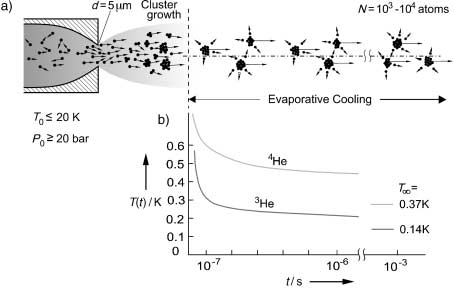
\includegraphics[width=0.6\textwidth]{../Images/jet_scketch.png}
	\caption[Scheme for a nozzle expansion]{ a) Schematic representation of the processes leading to the formation and subsequent cooling of helium droplets in a gas expansion. b) Calculated dependence of the droplet temperature on time for $^{4}He$ and $^{3}He$ droplets after they have left the cluster, taken from \cite{toennies_superfluid_2004}	}
	\label{img:jet}	
\end{figure}

\begin{figure}[h!]
\centering
	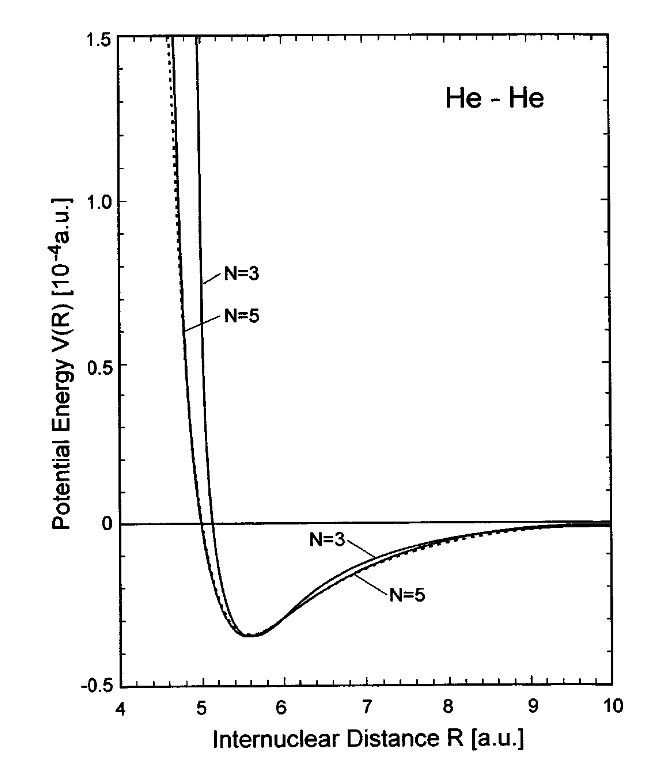
\includegraphics[width=0.5\textwidth]{../Images/waanderwaal_hehe.PNG}
	\caption[Waan der Wall He-He potential]{ Waan der Wals potential for He-He interaction}
	\label{img:WanderHe}
\end{figure}


When the Helium expands from the nozzel, its thermal energy is transform in kinetic energy of a supersonic flow field. After the expantion into the vacuum, the gas becomes supersaturated and condensations starts to occurs, creating the beam clusters. This clusters are made of atoms or moleulces held togueter by Wannder wals fores, in this case He-He interaction, that share the same kinetic vector. This means that the two particules travel as close and parallel to each other that a bonding is possible, see fig \ref{img:WanderHe}. From the reference frame of the cluster, each of its molecules are close to cero movments, in He this enhace the conditions to be liquid and in consecience superfluidity is achive  \cite{hagena_cluster_1972}.
 

There is no mathematical approach of the physics behind this cooling expansion but usually, Raleigh scattering measurements in combination with an empirical scaling law \cite{hagena_cluster_1972} are used to estimate the mean cluster size giving a certain degree of control over the cluster size distribution by adjusting the nozzle width and the source pressure. The droplet size distribution during supersonic expansion in the follows a log-normal distribution of the form \cite{harms_density_1998}.

\begin{equation}
p(N) = \frac{1}{\sqrt{2\pi}N \sigma} \exp  \left[- \frac{(ln(N/N_{0})^2}{2\sigma^2} \right]
\end{equation}
Where \textit{N} is the number of atom in the cluster, $\sigma$ is the distribution width and \textit{$N_{0}$} is the most likely numbers of atoms. Following it give a mean value.
\begin{align}
\bar N = \exp  \left(\mu+\frac{\sigma^2}{2} \right)
\end{align}
With a half width maxima of \cite{harms_density_1998}
\begin{align}
\sigma N_{\frac{1}{2}} = \exp \left( \mu - \sigma ^2 + \sigma \sqrt{2 ln(2)} \right) - \exp \left(  \mu - \sigma ^2 - \sigma \sqrt{2 ln(2)}  \right)
\end{align}

\begin{figure}[hbtp] \label{fig:ExpRegim}
\centering
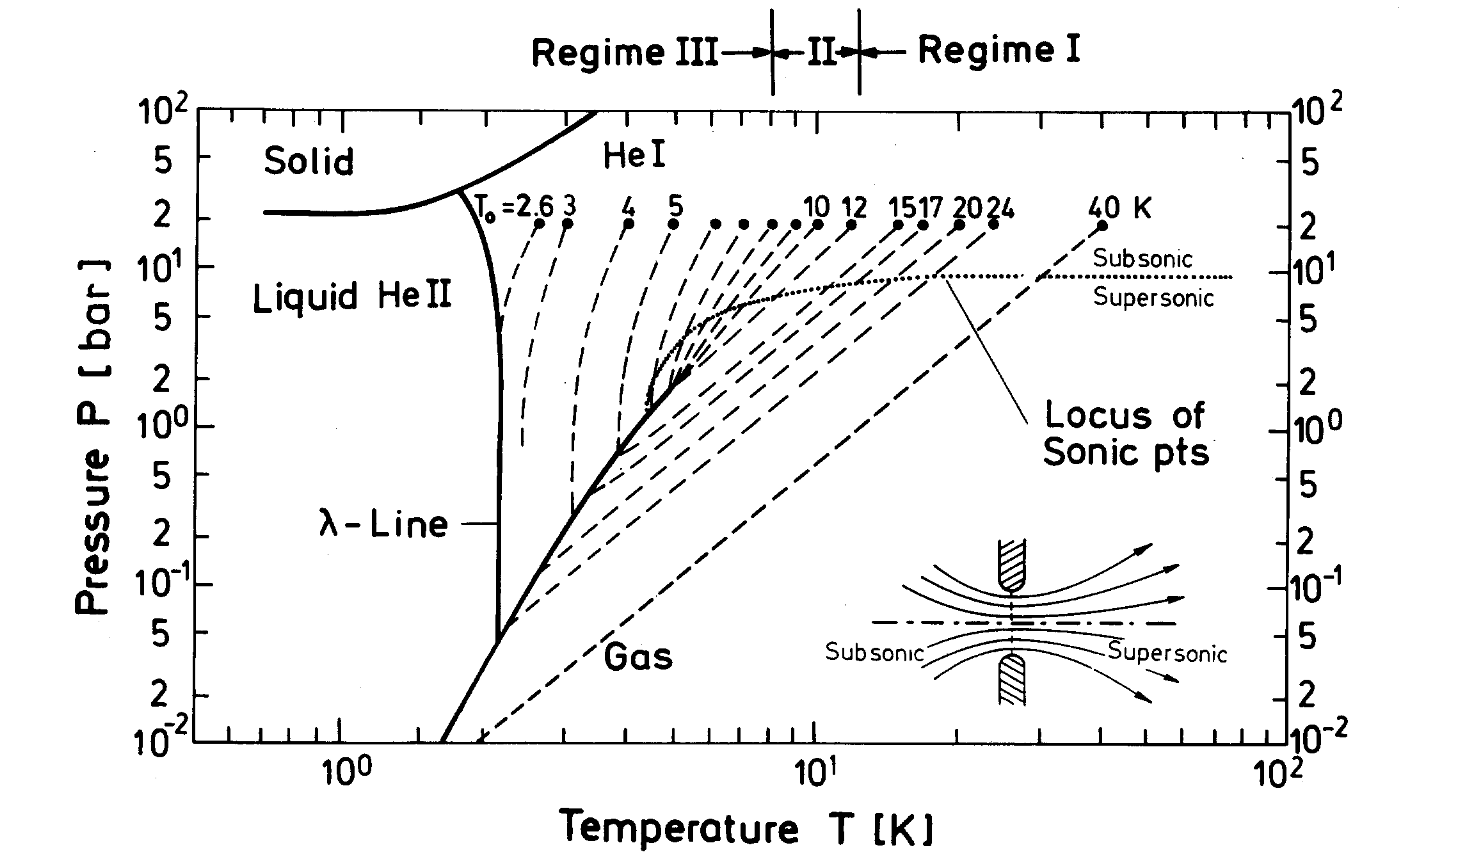
\includegraphics[width= 13 cm]{../Images/expansion_regimes.PNG}
\caption[Phase diagram for Expantion regimens]{Expansion regimes. Pressure-Temperatur phase diagram for $^{4}He$ for Nozzle beam expansions starting from a stagnation of 20 bar and a temperatures. As dicusse, quialitatively different behaivors are shown for the regime I - II and II where  starting in the gas phase,  near the phase trnasition respectivelly. taken from \cite{buchenau_mass_1990}. }
\end{figure}

As show in Figure \ref{fig:ExpRegim} The conditions in the He (pressure, temperature and nozzle size) in the free expansion will determine the characteristics of our final He beam. From Here three main regimes can be define.

Regime I or subcritical expansion, begins in the gas phase and leads to droplet formation via condensation. this is the case of most expansions since the pressure are located below the critical pressure $P_{c}$.
Regime II, also called as critical expansion, is basically  and interminable regime that includes all trajectories which are near the critical point, leading to random expansion and difficult control of the beam due the large fluctuations in density.
Regime III, the  supercritical expansion, starts at low temperatures where the He stops behaving as an ideal gas, expecting flashing or cavitation  breaking up the liquid drops jet. \cite{buchenau_mass_1990}

supercritial and subcritical regimes have been studies  in the las several years and  are clearly identified in the resulting size distributions. Figure \ref{img:dropletSize} shows that supercritical expansion forms large droplets (usuallz between $20-100 nm$ diameter) while a subcritical expansion is suited to generate small droplets (arround $5-10 nm$).  A simple relation that can be done to calculate the size or number of atom in a custer is using. \begin{equation}
r=N_{1/3} * \rho\angstrom
\end{equation}

Where $r$ is the radius of the beam, $\rho$ is the density, in thhis case of He $\rho =0.0022 \angstrom$ \cite{stringari_systematics_1987}, but this approximation is not exact due the variation Of He density at this temperatures. As expected in both regimens for creating larger helium nano droplets, higher helium pressure and lower nozzle temperature are used. For our experient a $5 \mu m$ nozzle was used at temperature oscillating between $11-15 K$, at pressure of $30 to 50$ bar.

\begin{figure}[hbtp]
\centering
\label{img:dropletSize}
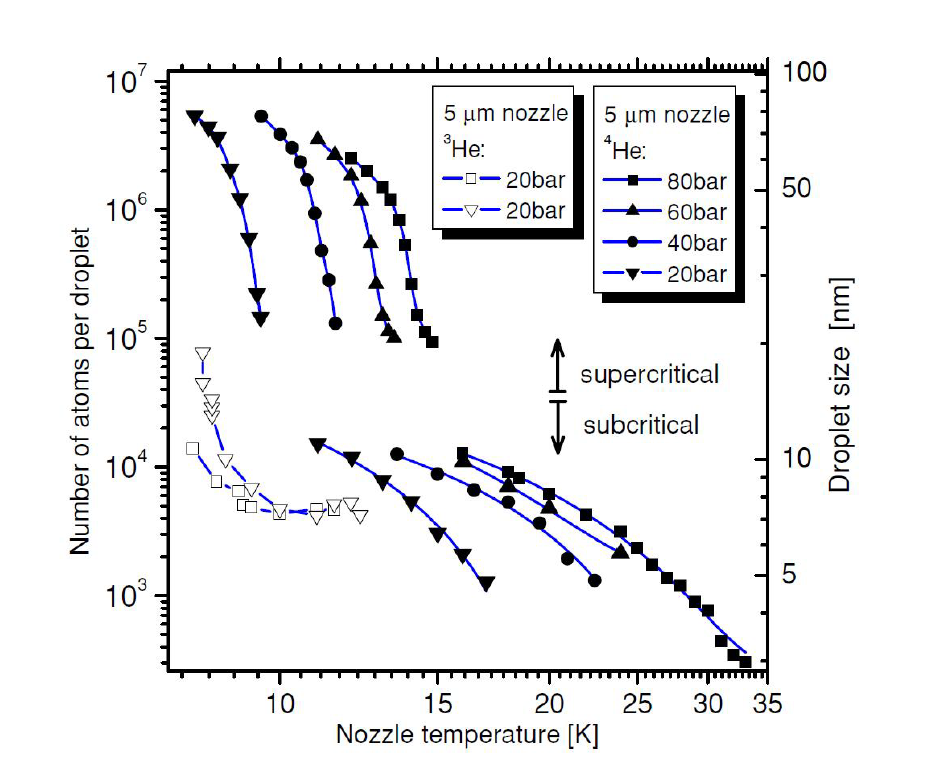
\includegraphics[scale=1]{../Images/sizes_regimen.PNG}
\caption{ Sizes of the $^{4}He$ droplets  as a function of nozzle temperature T and  pressures, based on \cite{toennies_spectroscopy_1998}, using a $5 \mu m$ nozzle. The su and super critical regimes are clearly diferenciated. Taken from \cite{stienkemeier_spsectroscopy_2006}}
\end{figure}


\subsubsection{Composite Clusters}

We can define a composite cluster or doped cluster, as a atom  bulk of one material that contains one or more different atomic elements. Usually in homogeneous clusters the main interest is their properties behaviour as a function of its size, but for doped clusters, the interaction between the atomic elements creates new degrees of freedom that makes more complex its behaviour. For example, the new composite will have different structural properties due its spatial distribution of different species. Hence, composite clusters exhibit a more diverse behaviour and offer more opportunities to study different properties of matter at the nano-scale.

Fhe first problem in composite cluster to overcome is how to create it. Two techniques can be used. The first one is the coexpansion of
a previously mixed gas \cite{tchaplyguine_variable_2004} or the He cluster is produced first and then crossed with an atomic beam of the dopping species.

The fisrst involve several thecnical probles due the  possible interaction of the two elements, the condensation ranges or even if they a likeble XXXXX materials or not. One of the most use thecniques, and the one used in this study is the one called "pick$-$up" thechnique \cite{gough_infrared_1985}. The idea is simple, as well as a snowball on its way down hill collects or "pick-up" more snow, the He cluster after been directional selected through a Skimmer  pass through a doping cell with a dopant gas at low densities ($10−2 Pa$)\cite{stienkemeier_spectroscopy_2006}. As result, the gass atoms that are along the droplet cross sections will be capture by the beam and travel with it. The probability for helium droplets to collect $k$ atoms or molecules via inelastic collisions depends on the length of the oven cell $l$, the cross section of the droplets $\sigma$, and the particle density inside the cell $n$.As $l$ and $\sigma$ reaming constant, varying the density in the doping cell results in a method to regulated the abundance of $k$, following the Poissonian statistics:

\begin{equation}
P_{k}(l,n,\sigma)=\dfrac{(ln\sigma)^{k}}{k!} e^{(-ln\sigma)}
\end{equation}
Two important properties of these relation can be infer: the maxima of
different cluster sizes  are equidistant, $n_{max}=\dfrac{k}{l\sigma}$ and that thee the exponential function in equation  becomes  nearly  1  for  small  particle  densities \cite{bunermann_modeling_2011}.



less than ≈100 ps.3 Of course, to trap a solute, its translational energy must fall below the
solvation energy in that time, not reach equilibrium with the droplet. Typical lengths of the
scattering cells are a few centimetres. The required partial pressure of molecules in the cell
has to be of the order of about 10−2 Pa, providing a maximum of singly doped droplets of
¯N
= 5000. Depending on the material of interest, different techniques are suitable to provide
the required vapour pressure inside the scattering cell. Gases or high vapour pressure liquids
and solids samples are directly introduced through room temperature capillaries. Higher
temperatures are often used to establish the required vapour pressure from bulk material inside
a heated cell. Temperatures exceeding 1500 K have been used in order to evaporate metals
[36]. Thermal radiation from the cell or heating is not a problem for the droplet beam because
dipole active transitions in helium require 20 eV of photon energy. In the same way, hightemperature
assemblies have been employed to dope radicals by means of pyrolysis [37]. In
this case, an effusive continuous beam of radicals efficiently dopes the helium droplets. 